% This chapter includes
% 3. Analysis procedures
%    3.1 Data sets and MC samples
%        3.1.X sub-sections for samples
%    3.2 Trigger
%    3.3 Physics objects reconstruction and identification
%        3.3.X sub-sections for physics objects

\chapter{Analysis Procedures}

In this chapter, the analysis procedures of the search for $Z'$ decaying into $Z$h in $llbb$ final state are reported. The data sets and Monte Carlo (MC) samples we used in this analysis will be indicated. Physics objects reconstruction and event selections are also introduced. Moreover, background yields and the effects of systematic uncertainties will be demonstrated in the end of this chapter.

\section{Monte Carlo Samples and Data sets}

\subsection{Signal MC}
As introduced in section 1.2.3, the signal hypothesis is HVT model B benchmark. The heavy resonance ($Z'$) is tested using a wide set of masses from 800 GeV to 2000 GeV, one masspoint every 100 GeV (Table~\ref{tab:TableSignalMC}). The signal is simulated by MadGraph5\_aMC$@$NLO\cite{MG5} in LO mode, as a narrow spin-1 neutral resonance and is forced to decay in the $Z'\rightarrow Zh\rightarrow llqq$ channel. Showering and hadronization are performed with PYTHIA6\cite{PYTHIA}.
\begin{figure}[hbtp]
  \begin{center}
    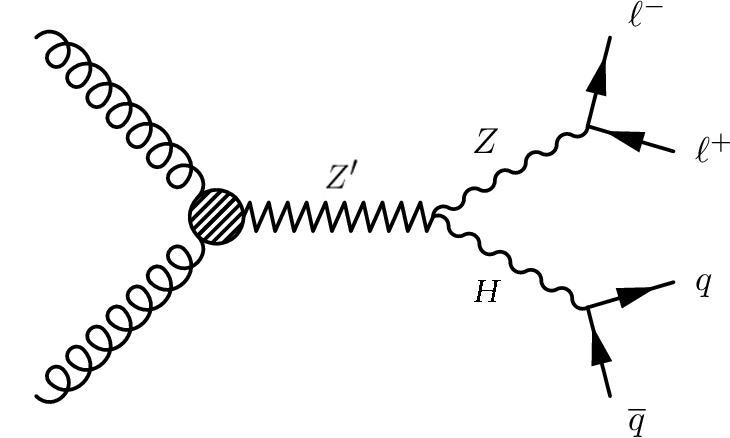
\includegraphics[width=0.4\textwidth]{figure/CH3/ZPrimeTo2l2q.png}
  \end{center}
  \caption{\label{fig:ZPrime2l2q}Feynman diagram for $Z'\rightarrow Zh \rightarrow 2l2q.$}
\end{figure}
\begin{center}
  \begin{table}
    \begin{center}
      \begin{tabular}{|c|c|c|}
        \hline
        Sample & Number of Processed Events & $\sigma_{LO}$(pb) \\ \hline
        ZPrime\_ZH\_lljj\_M800-MADGRAPH & 10710 & 0.00685367 \\ \hline
        ZPrime\_ZH\_lljj\_M900-MADGRAPH & 10209 & 0.00485861 \\ \hline
        ZPrime\_ZH\_lljj\_M1000-MADGRAPH & 19997 & 0.003263 \\ \hline
        ZPrime\_ZH\_lljj\_M1100-MADGRAPH & 9370 & 0.00217483 \\ \hline
        ZPrime\_ZH\_lljj\_M1200-MADGRAPH & 10710 & 0.00145484 \\ \hline
        ZPrime\_ZH\_lljj\_M1300-MADGRAPH & 9369 & 0.000979745 \\ \hline
        ZPrime\_ZH\_lljj\_M1400-MADGRAPH & 10497 & 0.000664783 \\ \hline
        ZPrime\_ZH\_lljj\_M1500-MADGRAPH & 19999 & 0.000454339 \\ \hline
        ZPrime\_ZH\_lljj\_M1600-MADGRAPH & 8950 & 0.000312541 \\ \hline
        ZPrime\_ZH\_lljj\_M1700-MADGRAPH & 9369 & 0.000216282 \\ \hline
        ZPrime\_ZH\_lljj\_M1800-MADGRAPH & 10708 & 0.000150398 \\ \hline
        ZPrime\_ZH\_lljj\_M1900-MADGRAPH & 10498 & 0.000105039 \\ \hline
        ZPrime\_ZH\_lljj\_M2000-MADGRAPH & 19999 & 7.36377e-05 \\
        \hline
      \end{tabular}
    \end{center}
    \caption{\label{tab:TableSignalMC}Signal samples used in the analysis.}    
  \end{table}
\end{center}
\newpage
\subsection{Background MC}
Since we are looking for new resonances decaying in semi-leptonic final state, the background samples of this analysis are originated by all SM events with two leptons and at least one jet as final state. The dominant background contribution is the produciton of Z boson with jets. This Z+jets sample is produced by MADGRAPH. In the matrix element level, the Z boson is forced decaying into two leptons, and further this sample is divided into two samples depending on the Z $p_{T}$, higher than 100 GeV or between 70 and 100 GeV. The contribution of events with Z $p_{T}$ less than 70 GeV is negligible due to further cut on the objects $p_{T}$ in the selection criteria.

The second dominant source of background is $t\bar{t}$ production. Both of the two top quarks decay into all leptonic final state (top decays into a W boson and a b quark first) which gives two leptons, neutrinos and two b-jets. This sample is generated by POWHEG\cite{POWHEG}.

Other sources of background considered are SM di-boson productions (WW, WZ and ZZ) generated by PYTHIA6. All the background samples are required to pass phase-space cuts, $p_{T}^{ll} > $60 GeV and 60$ < M_{ll} < $120 GeV. Related statistics are reported in Table~\ref{tab:TabBkgMC}.

\begin{center}
  \begin{table}[h]
    \begin{center}
      \begin{tabular}{|c|c|c|}
        \hline
        Sample & Number of Processed Events & $\sigma_{NLO}$(pb) \\ \hline
        DYJetsToLL\_PtZ-70To100 & 11764538 & 63.5 \\ \hline
        DYJetsToLL\_PtZ-100 & 12511326 & 39.4 \\ \hline
        TTTo2L2Nu2B & 10783509 & 25.8 \\ \hline
        WW & 7759752 & 56.0 $\pm$ 2.3 ($\pm$ 0.3) \\ \hline
        WZ & 9910267 & 22.4 \\ \hline
        ZZ & 9769891 & 7.6 $\pm$ 0.3 ($\pm$ 0.3)\\
        \hline
      \end{tabular}
    \end{center}
    \caption{\label{tab:TabBkgMC}Background samples used in the analysis.}    
  \end{table}
\end{center}

\subsection{Data Samples}
In this analysis, the full CMS data collected in 2012 is used, corresponding to the integrated luminosity of 19.7 fb$^{-1}$ at center-of-mass energy $\sqrt{s} = $8 TeV. For each lepton channel, there are four datasets. All datasets are collected with a double muon or a double electron trigger, as explained in detail in the next section. The trigger algorithm employed for the electron samples doesn't use any information from the tracker but only the energy deposite in the ECAL. This expedient is implemented in order to avoid any possible inefficiencies due to the presence of two tracks very close to each other when the Z is highly boosted and its decay products are very collimated. Such a trigger is contained in the Photon/DoublePhotonHighPt dataset. The full dataset names are listed in Table~\ref{tab:TabDataSet}.

\begin{center}
  \begin{table}[h]
    \begin{center}
      \begin{tabular}{|c|c|}
        \hline
        AOD Sample & Luminosity (pb$^{-1}$) \\ \hline
        DoubleMu/Run2012A-22Jan2013-v1 & 876.225 \\ \hline
        DoubleMuParked/Run2012B-22Jan2013-v1 & 4409 \\ \hline
        DoubleMuParked/Run2012C-22Jan2013-v1 & 7017 \\ \hline
        DoubleMuParked/Run2012D-22Jan2013-v1 & 7369 \\ \hline
        Photon/Run2012A-22Jan2013-v1 &  876.225 \\ \hline
        DoublePhotonHighPt/Run2012B-22Jan2013-v1 & 4412 \\ \hline
        DoublePhotonHighPt/Run2012C-22Jan2013-v1 & 7055 \\ \hline
        DoublePhotonHighPt/Run2012D-22Jan2013-v1 & 7369 \\
        \hline
      \end{tabular}
    \end{center}
    \caption{\label{tab:TabDataSet}Data sets used in this analysis.}    
  \end{table}
\end{center}

\section{Trigger}
Since the final state contains two same flavour leptons and at least one jet, we perform this analysis on the DoubleMu and Photon/DoublePhotonHighPt datasets. The first dataset is triggered by two muons, the second one is triggered by two eletrons. These triggers are:
\begin{itemize}
\item HLT\_Mu22\_TkMu8* (for DoubleMu datasets)
\item HLT\_DoubleEle33\_* (for Photon/DoublePhontonHighPt datasets)
\end{itemize}

The muon trigger has a double $p_{T}$ threshold, requires leading muon $p_{T}$ greater than 22 GeV and sub-leading muon $p_{T}$ greater than 8 GeV. Differently, the double electron trigger requires a higher threshold of 33 GeV to electrons. The trigger efficiencies are close to 1 in both cases.

\section{Physics Objects}

\subsection{Muon}
\subsection*{Reconstruction}
The muon reconstruction algorithm at CMS takes advantage of the redundancy of detection methods. Muon tracks are first reconstructed independently in the inner tracker (tracker track) and in the muon system (standalone track). Based on these objects, two reconstruction approaches are used\cite{MuonReco}:
\begin{itemize}
\item $Globol~Muon$ (outside-in): Starting from a standalone track, this algorithm finds a best tracker track to match the standalone track. Then, the fit of the track is repeated using the hits both in the tracker and in the muon system\cite{KF}. The resulting object is called a $Global~Muon$. At large transverse momentum ($p_{t} > $200 GeV), the global muon fit can improve the momentum resolution compared to the tracker only fit.
\item $Tracker~Muon$ (inside-out): A tracker muon is reconstructed by an opposite direction from a global muon. In this approach, all tracker tracks with $p_{T} >$ 0.5 GeV and the total momentum $p >$ 2.5 GeV are considered as possible muon candidates. The extrapolation to the muon system takes into account the magnetic field, average expected energy losses, and multiple scattering in the detector material. If at least one muon segment matches the extrapolated track, the corresponding track track qualifies as a $Tracker~Muon$. This algorithm is useful for low-$p_{T}$ muons that are not fully penetrate the muon system, and therefore only register a few hits
\end{itemize}

If no match is found when extrapolating outside-in, the standalone track is stored as a $Stanalone~Muon$. This happens only for less than 1\% of the muons produced in a collison, and the reconstruction efficiency is about 99\% for the muon which carries enough high momentum within detector coverage\cite{MuonReco}.

\newpage
\subsection*{Identification}
We use both tracker muons and global muons in this analysis. To identify muons from the signal, the muons must pass one of these two off-line selections, high$-p_{T}$ muon ID or tracker-based muon ID\cite{MuonID}. The requirements are listed as follows:\\

High-$p_{T}$ muon ID
\begin{itemize}
\item Muon identified as a $Global~Muon$.
\item Number of muon hits in the global track $> 0$.
\item Number of matched muon stations $> 1$.
\item Number of pixel hits $> 0$.
\item Number of tracker layer with hits $> 8$.
\item Transverse impact parameter $d_{xy} < 0.2$ cm.
\item Longitudinal impact parameter $d_{z} < 0.5$ cm.
\item Relative error on the track transverse momentum $\sigma_{p_{T}}/p_{T} < 0.3$.\\
\end{itemize}

In the tracker-based muon ID, the muon has to be identified as a $Tracker~Muon$, and the requirement of muon hits in the global track is removed. Other requirements are the same.

An additional useful variable for lepton identification is the isolation. It is defined as the scalar sum of the $p_{T}$ of the reconstructed objects within a cone (typical size is $\Delta R=0.3$) space around the lepton track but excluding the $p_{T}$ of the lepton itself. Moreover, the relative isolation is defined as isolation divided by the lepton $p_{T}$ ($I_{rel} = Iso/p_{T}^{lep}$). The relative isolation is more frequently used in the modern analysis.

In this analysis, a modified isolation criteria is used. The two muons originated from boosted Z decay are close to each other, and consequently the presence of another muon in the isolation cone could break the function of this variable. In order to solve this problem we use a tracker-based isolation relative quantity, explicitely removing the momentum flow from any other muon passing our muon selection. Moreover, a tracker-based isolation is well motivated also by two additional aspects: it is more independent of pile up (pile-up tracks tipically do not match the primary vertex) and does not include possible muon radiation. Finally, the modified requirement is $I_{rel}^{mod} < 0.1$.\\

\begin{table}[h]
  \begin{center}
    \begin{tabular}{|l|c|c|}
      \hline
      Variable & High-$p_{T}$ & Tracker-based \\ \hline
      Muon type & Global muon & Tracker muon \\
      Muon hits in global track & $\geq$ 1 & - \\
      Muon stations matched & $\geq$ 2 & $\geq$ 2 \\
      $d_{xy}$ & $<$ 0.2 cm & $<$ 0.2 cm\\
      $d_{z}$ & $<$ 0.5 cm & $<$ 0.5 cm\\
      Pixel hits & $\geq$ 1 & $\geq$ 1 \\
      Tracker layers & $\geq$ 8 & $\geq$ 8 \\
      $\sigma_{p_{T}}/p_{T}$ & $<$ 0.3 & $<$ 0.3 \\ \hline
      $I_{rel}^{mod}$  & $<$ 0.1 & $<$ 0.1 \\
      \hline
    \end{tabular}
    \caption{\label{tab:MuonIDtable} Summary of the muon ID selection criteria.}
  \end{center}
\end{table}

\newpage
\subsection{Electron}

\subsection*{Reconstruction}
Electrons are reconstructed from energy deposits in the ECAL matched to tracks reconstructed in the silicon tracker. They have less distinguishable signatures than muons in the detector due to the jet induced background in ECAL. Therefore, to reconstruct an election, it's essential to find a briliant way to match the infomation acquired in both tracker and ECAL.

\subsection*{Clustering}
For every single hit from an electron in ECAL, approximately 94\% of energy is contained in 3$\times$3 crystals and 97\% in 5$\times$5 crystals. To form a cluster, crystals with $E_{T} > 1$ GeV is picked as seeds. Then starting from seed crystal, dominos of size 1$\times$3 or 1$\times$5 are created in $\eta-\phi$ plane. If the energy of these dominos exceed 0.1 GeV threshold, thus added up the energy of dominos along the $\phi$ direction.

Moreover, the effects of conversion process and bremsstrahlung radiation must be taken into account to reconstruct the electron energy more precisely. The concept of electron superclustering is to collect the energy of photons from bremsstrahlung radiation along the $\phi$ direction with fixed $\eta$ width of the seed crystal. The technical details of the supercluster can be found in\cite{eleSC}.

\subsection*{Tracking}
There are several steps to reconstruct electron tracks in CMS experiment. The hit on the pixel and the tracker are reconstructed in the first step. The second step is to find the seed of tracks by matching at least two hits in pixel detector. Lst step is to fit the trajetory starting from the seed. To perform this fit, the Gaussian-sum filter (GSF) algorithm is used\cite{GSF}. In GSF algorithm, the energy loss probability density function is constructed by multiple Gaussian functions. Finally, the electrons are built by matching the superclusters to the GSF tracks. Reconstruction efficiencies for electrons $E_{T} > 20$ GeV are generally above 95\% in EB and 90\% in EE\cite{eleRecoEff}.

\subsection*{Identification}
The electron identification used in this analysis is based on HEEPv4.1\cite{HEEP}. As what we did for the muon id, we need to modify the isolation definition again because of the small $DeltaR$ between two electrons. The requirements are listed as follows:\\

Modified HEEPv4.1 electron ID
\begin{itemize}
\item Transversal supercluster energy $>$ 35 GeV.
\item Pseudorapidity of supercluster $\eta_{SC} < 1.442$ for barrel electrons, or $1.56 < \eta_{SC} < 2.5$ for endcap electrons.
\item Have either $E_{2\times 5}/E_{5\times 5} > 0.94$ or $E_{1\times 5}/E_{5\times 5} > 0.83$.
\item Ratio of HCAL deposit energy to ECAL deposit energy (Fig.~\ref{fig:E5X5}) smaller than 0.5.
\item Number of inner layer lost hits smaller than 2.
\item Have $d_{xy} < 0.02$ cm for barrel electrons, or $d_{xy} < 0.05$ cm for endcap electrons.\\
\end{itemize}

As what we did for the muon id, by the same reason we need to modify the isolation definition again. In this case there are three isolation variableshave to be changed.

\begin{itemize}
\item Modified track isolation is required to lower than 5 GeV. This variable is defined as the scalar $p_{T}$ sum of the tracks within a $\Delta R$ = 0.3 cone around the electron, and excluding the $p_{T}$ of another electron which passes the above selections and its track is inside the cone.
\item The electromagnetic calorimeter isolation $I_{ECAL}$ is defined as the scalar sum of $E_{T}$ of the crystals in a $\Delta R$ = 0.3 cone around the particular electron (an inner area of full-width 3 crystal), excluding a 4 crystals $\Delta R$ cone around any other electron. The dimension of the ECAL crystals corresponds roughly at $\Delta R \sim 0.01 \textup{ to } 0.02$. The threshold of $I_{ECAL}$ is varying with the electron transverse energy.
\item The hadronic calorimeter isolation $I_{HCAL}$ is defined as the scalar sum of $E_{T}$ of the HCAL caloTowers with a center in a $\Delta R$ = 0.3 cone around the electron, excluding those lying within $\Delta R$ = 0.15 of the electron itself and of any other electron\cite{CMS_AN_2012-168}. The threshold of this variable also varies with the electron transverse energy.
\end{itemize}
\newpage
\begin{figure}[hbtp]
  \begin{center}
    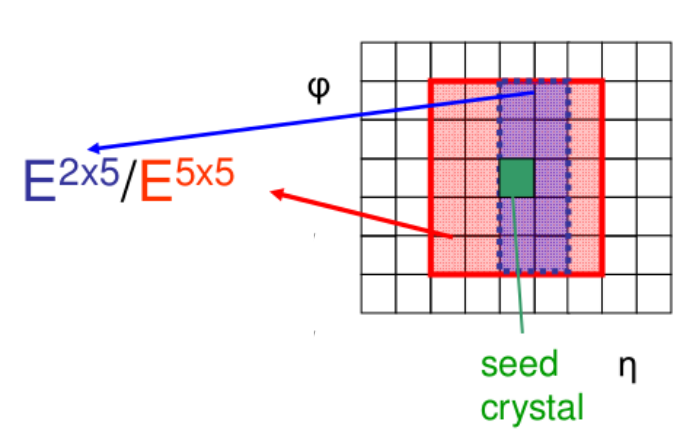
\includegraphics[width=0.5\textwidth]{figure/CH3/E5X5.png}
  \end{center}
  \caption{\label{fig:E5X5}Example of the $E_{2\times5}/E_{5\times5}$ computation in the ECAL crystals. $E_{i \times j}$ is the energy contained in a $i \times j$ block around the seed crystal (defined as the highest deposit of the energy of the cluster).}
\end{figure}

\begin{table}[hbtp]
  \begin{center}
    \begin{tabular}{|l|c|c|}
      \hline
      Variable & Barrel & Endcap \\\hline
      $E_{T}$ & $>$ 35 GeV & $>$ 35 GeV \\
      $|\eta_{SC}|$ & $|\eta_{SC}|$ $<$ 1.442 & 1.56 $<$ $|\eta_{SC}|$ $<$ 2.5 \\
      H/E & $<$ 0.05 & $<$ 0.05 \\ 
      $E_{2\times5}/E_{5\times5}$ & $>$ 0.94 & - \\
      & or $E_{1\times5}/E_{5\times5}$ $>$ 0.83 & \\ 
      Inner Layer Lost Hits & $<=$ 1 & $<=$ 1 \\
      $|d_{xy}|$ & $<$ 0.02 cm & $<$ 0.05 cm\\
      \hline
      $Iso_{Trk}^{mod}$  & $<$ 5 GeV& $<$ 5 GeV\\
      \hline
      $Iso_{Ecal, Hcal}^{mod}$  & $<$ 2 GeV + 0.03$E_{T}$ & $<$ 2.5 GeV for $E_{T} <$ 50 GeV \\
      & & $<$ 2.5 GeV + 0.03$E_{T}$ for $E_{T} >$ 50 GeV \\
      \hline
    \end{tabular}
    \caption{\label{tab:EleIDtable} Summary of the modified HEEPv4.1 electron ID.}
  \end{center}
\end{table}

\newpage
\subsection{Jet}
Since gluons and quarks cannot exist in free state due to the color confinement\cite{confinement}, they fragment into hadrons. The result of this fragmentation (or called the "hadronization") is a jet of particles depositing energy in the detectors.

\subsection*{Reconstruction}
Jet clustering algorithms are among the main tools for analyzing data from hadronic collisions. In this section, a extensively used clustering algorithm called "sequential recombination algorithm"\cite{AKalgo,CAalgo1} will be introduced. At first, events are reconstructed using the particle flow algorithm (PF)\cite{PFalgo}, which attempts to identify and measure all the stable particles in a collision by combining information from all the sub-detectors. The PF algorithm categorizes all particles into five types: muons, electrons, photons, charged and neutral hadrons. The resulting particle flow candidates are passed to the anti-k$_{T}$ (AK)\cite{AKalgo} or Cambridge/Aachen (CA)\cite{CAalgo1,CAalgo2} jet clustering algorithms to create jets (AK and CA are two commonly used branches of sequential recombination algorithms).

The jet clustering algorithms are implemented as follows:

\begin{align}
  \label{eq:jetCluster}
  &d_{iB}=p_{T,i}^{2p}\nonumber \\
  &d_{ij}=min(p_{T,i}^{2p}, p_{T,j}^{2p})\frac{\Delta R_{i,j}^{2}}{R^{2}}
\end{align}

In Eq.~(\ref{eq:jetCluster}), the pair of objects ( i , j ) denote two input candidate particles to the algorithm. $\Delta R_{ij}$ is the spatial distance between the two objects, and $R$ is the typical cone size of the jet. The parameter $p$ corresponds to different catagories of algorithms and will be introduced in the later paragraph.

The clustering proceeds by comparing the value of the two quantities, $d_{iB}$ and $d_{ij}$. If $d_{ij} > d_{iB}$, the algorithm will look for another possible combination of ( i , j ).  If $d_{ij} < d_{iB}$, the 4-momentum of object i will merge into j, and then the object j forms a pseudo-jet, but the algorithm will not stop looking for a new object until all particles are clustered into jet.

The parameter $p$ can be chosen as follows:

\begin{itemize}
\item $p = 0$ : Cambridge/Aachen algorithm;
\item $p = -1$ : Anti-$k_{T}$ algorithm;
\end{itemize}

The difference between CA/AK algorithms is clear, CA algorithm is only considering the spatial distance of the two candidate objects (if $\Delta R_{ij} < R$, merged). In the case of anti-k$_{T}$ algorithm, $p_{T}$ of the object presents as a weight for the distance.

The anti-k$_{T}$ algorithm have better energy calibration, while the CA algorithm was found to be more efficient at finding hard subjets within the jets in simulation-based studies\cite{CAalgo3}. Therefore the CA jets are used in this analysis to identify events containing hadronically-decaying Higgs bosons.

\subsection*{Identification}
As disscussed in the previous section, this analysis use the Cambridge/Aachen algorithm with a cone radius of R = 0.8 for the identification of jets (CA8 jets). Furthermore, jets are required to pass the following loose identification criteria\cite{JetID,JetID2}:\\

Loose JetID ($>$ 99\% efficiency)
\begin{itemize}
\item Muon energy fraction smaller than 0.99
\item Photon energy fraction smaller than 0.99
\item Charged electromagnetic energy fraction smaller than 0.99
\item Neutral hadron energy fraction smaller than 0.99
\item Charged hadron energy fraction larger than 0
\item Number of constituent particles larger than 1
\end{itemize}

For the "charged" variables, $\eta < 2.4$ requirement are also applied, since there is no track coverage outside of this region, whereas the "neutral" variables extend to the whole $\eta$ region.

\subsection{Jet Grooming Algorithms and Pruned Jet Mass}

The jet mass is the main observable in distinguishing a boson-jet from a QCD jet. Jet grooming aims to suppress uncorrelated underlying events and pile-up radiation from the target jet, and improves the discrimination by pushing the jet mass for QCD jets towards lower values while mantaining the jet mass for boson-jets around the boson-mass\cite{AN-12-137,AN-13-072}.
